% =====================================================================
%  sections/sec6.tex —— 6 由六维 A_{k-1} 理论得到的 AD 点（原文 pp.31–46）
% =====================================================================
\section{由六维 $A_{k-1}$ 理论得到的 AD 点}
\label{sec:ak}

\subsection{非正则奇点的选取}
\label{sec:6.1}

\routenote{原文 pp.31--33。本小节走反证：设奇点有两个 block、第二个 block 的维数 $k_2>1$，用「高阶极点的参数只能充当耦合常数与质量」定出最小算子的维数 $[v]$；再由 $[v]\le 1$ 与斜率顺序冲突，把这一类排除。剩下的只有两个 block 且 $k_2=1$，由此得到 Type I、Type II、Type III 三类奇点。}

现在从六维 $A_{n-1}$ 理论出发，把它紧致化在带非正则奇点的黎曼面上。首先要弄清：定义四维 SCFT 究竟需要哪一类非正则奇点。非正则奇点个数的分析同上一节：球面上可以只有一个非正则奇点，也可以在南北两极各放一个，即一个非正则奇点加一个正则奇点。在 $A_1$、$A_2$ 的情形，各类非正则奇点都能定义四维 SCFT。秩更高的群则不同：并非每个非正则奇点都能定义四维 AD 理论。

关键在于：高阶极点的参数应当充当耦合常数。因此，若 Seiberg--Witten 曲线中的某个算子只由这些参数构成，它的标度维数就必须小于一；换言之，这些项不能含有 Higgs 场的正则项给出的部分。这个条件对可用于寻找 SCFT 的非正则奇点类型施加了很强的限制。

非正则奇点由一串斜率确定，用这串斜率可以画出牛顿多边形。斜率按 $\lambda_1>\lambda_2>\cdots>\lambda_l$ 排列，其中 $\lambda_i=r_i-2$，$r_i$ 是非正则奇点中第 $i$ 个 block 的最大极点阶。先取 $\lambda_1=n_1+j_1/k_1$，其中 $j_1<k_2$、$n_1\ge 2$；这个 block 的领头阶矩阵取如下形式（奇点放在 $z=\infty$）：
\begin{equation}
B_1 = z^{n_1-2+j_1/k_1}\diag(1,\ \omega,\ \cdots,\ \omega^{k_1-1}) .
\label{eq:6.1}\tag{6.1}
\end{equation}
\typo{原文 p.32 的条件 $j_1<k_2$ 与 (3.15) 的 $0<j_i\le k_i$ 不协调。此处限定的是第一个 block 的分数部分，应为 $j_1<k_1$。}

这个 block 决定了各算子的标度维数，奇点处的 Seiberg--Witten 曲线为
\begin{equation}
x^n + x^{n-k_1}z^{k_1n_1-2k_1+j_1} = 0 ,
\label{eq:6.2}\tag{6.2}
\end{equation}
于是 $z$ 与 $x$ 的标度维数为
\begin{equation}
[z] = \frac{k_1}{k_1n_1-k_1+j_1},\qquad
[x] = \frac{k_1n_1-2k_1+j_1}{k_1n_1-k_1+j_1} .
\label{eq:6.3}\tag{6.3}
\end{equation}
\typo{原文 p.32 的 (6.2) 与 (6.4) 写作 $x^n$，这里的指数实为规范群的秩；原文从第 \ref{sec:6.1.1} 小节起改用 $k$。同样的滑移还见于 p.31 开头的「六维 $A_{n-1}$ 理论」——本节标题与后文都用 $A_{k-1}$。译文照录。}

现在打开第二个 block 对应的形变。该 block 的维数为 $k_2>1$，极点阶为 $r_2=n_1+j_2/k_2<r_1$（取 $n_2=n_1$，使 $[v]$ 的标度维数尽可能小），且 $j_2/k_2<j_1/k_1$。SW 曲线形如
\begin{equation}
\begin{aligned}
x^n &+ x^{n-k_1}z^{k_1n_1-2k_1+j_1}
+ x^{n-(k_1+k_2)}z^{k_1n_1-2k_1+j_1}\\
&\times\bigl(z^{k_2n_1-2k_2+j_2}+\cdots+vz^{(k_2-1)(n_1-2)+j_2-1}+\cdots\bigr) = 0 .
\end{aligned}
\label{eq:6.4}\tag{6.4}
\end{equation}
这里 $v$ 是只由高阶极点系数构成的最小算子，把谱曲线显式展开即可看出；它的标度维数由式 (6.3) 定出：
\begin{equation}
[v] = k_2[x]-\bigl((k_2-1)(n_1-2)+j_2-1\bigr)[z]
= \frac{(n_1-1)k_1+k_2j_1-k_1j_2}{k_1n_1-k_1+j_1} .
\label{eq:6.5}\tag{6.5}
\end{equation}
这个算子维数不得大于一，因为它必须充当耦合常数或质量。于是
\begin{equation}
[v]\le 1 \ \to\ k_2j_1-k_1j_2\le j_1
\ \to\ \frac{j_1}{k_1}\le\frac{j_2}{k_2-1}
\ \to\ \frac{j_1}{k_1}<\frac{j_2}{k_2} .
\label{eq:6.6}\tag{6.6}
\end{equation}
这与假设 $j_1/k_1>j_2/k_2$ 矛盾。

\zhnote{[译者按（无外部依据）：(6.6) 的末一步推不出来。当 $k_2>1$ 时总有 $j_2/(k_2-1)>j_2/k_2$，所以 $j_1/k_1\le j_2/(k_2-1)$ 并不能与 $j_1/k_1>j_2/k_2$ 冲突。原文此处的矛盾论证有缺口，下文结论照录原文。]}

\begin{figure}[tbp]
\centering
% Figure 12 -- graphic form of the Seiberg-Witten curve
\begin{tikzpicture}[x=1pt,y=1pt,scale=1.08,transform shape,>=stealth,line width=0.5pt]
  % ---- axes ----
  \draw (52.4,8.6) -- (52.4,175.3);
  \draw (4.6,56.4) -- (230.5,56.4);
  % ---- Newton-polygon-like outline ----
  \draw (99.6,56.0) -- (99.6,139.7) -- (147.5,115.5) -- (147.2,56.0);
  \draw (147.5,115.5) -- (206.7,56.2);
  % ---- k1, k2 brackets ----
  \draw (99.4,50.3) -- (117.9,50.4) -- (123.7,44.1) -- (129.7,50.6) -- (141.6,50.3);
  \draw (146.8,50.3) -- (171.3,50.4) -- (177.1,44.1) -- (183.0,50.6) -- (206.8,50.3);
  % ---- h1, h2 markers ----
  \draw (93.9,91.6) -- (81.9,139.8);
  \draw (93.9,92.3) -- (82.0,62.0);
  \draw (141.3,116.0) -- (135.3,85.7);
  \draw (141.3,62.0) -- (135.2,86.4);
  % ---- distinguished points ----
  \fill (82.0,145.3) circle[radius=1.85pt];
  \fill (70.1,151.2) circle[radius=1.85pt];
  % ---- labels ----
  \node[inner sep=0pt] at (181.25,35.6) {\fontsize{9}{11}\selectfont$k_1$};
  \node[inner sep=0pt] at (121.95,35.6) {\fontsize{9}{11}\selectfont$k_2$};
  \node[inner sep=0pt] at (127.95,88.9) {\fontsize{9}{11}\selectfont$h_1$};
  \node[inner sep=0pt] at (74.55,94.85) {\fontsize{9}{11}\selectfont$h_2$};
\end{tikzpicture}

\caption{由非正则奇点定义的 SW 曲线的图形。该奇点的领头阶矩阵含大小为 $k_1$、$k_2$、… 的 block。}
\label{fig:12}
\end{figure}

剩下的唯一可能是只有两个 block，且 $k_2=1$。此时领头阶矩阵为
\begin{equation}
\Phi = z^{n+\frac{j}{k-1}-2}\diag(0,\ 1,\ \omega,\ \cdots,\ \omega^{(k-1)-1}) .
\label{eq:6.7}\tag{6.7}
\end{equation}
因此，可用于定义 AD 理论的非正则奇点分类如下：
\begin{enumerate}
  \item Type I 奇点：
\begin{equation}
\Phi = z^{n+\frac{j}{k}-2}\diag(1,\ \omega,\ \cdots,\ \omega^{n-1}),\qquad 0<j\le k .
\label{eq:6.8}\tag{6.8}
\end{equation}
  \item Type II 奇点：
\begin{equation}
\Phi = z^{n+\frac{j}{k-1}-2}\diag(0,\ 1,\ \omega,\ \cdots,\ \omega^{(n-1)-1}),\qquad 0<j<k-1 .
\label{eq:6.9}\tag{6.9}
\end{equation}
\typo{原文 p.33 的 (6.8) 把对角元写到 $\omega^{n-1}$，应为 $\omega^{k-1}$；(6.9) 写到 $\omega^{(n-1)-1}$，应为 $\omega^{(k-1)-1}$，依据是 (6.7) 的同型写法 $\omega^{(k-1)-1}$。矩阵的阶由规范群秩 $k$ 定，与极点阶的整数部分 $n$ 无关。}
  \item Type III 奇点：可以考虑上述非正则奇点的退化。有两种情形。

  \textbf{Case 1：}极点阶为整数。此时奇点由一列杨图 $Y_n\subseteq Y_{n-1}\cdots\subseteq Y_1$ 指定，其中 $Y_{j-1}$ 由 $Y_j$ 的每一列进一步分拆得到。

  \textbf{Case 2：}极点阶为分数。此时只需确定分拆，它由牛顿多边形上的整点定出。例如，若一般的奇点为
\begin{equation}
\Phi = z^{n-2+\frac{2}{4}}\diag(1,\ \omega,\ \cdots,\ \omega^{3}) ,
\label{eq:6.10}\tag{6.10}
\end{equation}
牛顿多边形的边界上就会出现一个整点。若选取这个点，领头阶奇点可退化为
\begin{equation}
A_0 = z^{n-2+\frac{2}{4}}\diag(1,\ -1,\ 1,\ -1) .
\label{eq:6.11}\tag{6.11}
\end{equation}
\zhnote{[依据：(6.10) 与 (6.11) 的对照。] (6.11) 中的 $A_0$ 是退化后领头阶矩阵的名字，并不是一个叫 $A_0$ 的理论，与六维 $A_{n-1}$ 理论的 $A$ 记号无关。}
\end{enumerate}

下面略谈应与物理考虑相匹配的几何量。例如，库仑分支的维数应与 Hitchin 纤维化的底的维数相等，即 Hitchin 模空间维数的一半。质量参数则基本由一阶极点系数的形式定出。

以上列表穷尽了可用于定义 SCFT 的全部非正则奇点。下面逐一细看。

\subsubsection{Type I SCFT：$(A_{k-1},A_{N-1})$ 理论}
\label{sec:6.1.1}

把六维 $A_{k-1}$ 理论紧致化到带 Type I 非正则奇点的球面上。只打开领头阶矩阵时，奇点处四维 SCFT 的 Seiberg--Witten 曲线为
\begin{equation}
x^k+z^N = 0 .
\label{eq:6.12}\tag{6.12}
\end{equation}
这个奇点的极点阶为 $r=N/k+2$，并用标度不变性把 $z^N$ 的系数定为 1。$x$ 与 $z$ 的标度维数为
\begin{equation}
[x] = \frac{N}{N+k},\qquad [z] = \frac{k}{N+k} .
\label{eq:6.13}\tag{6.13}
\end{equation}
文献 \cite{17} 把这个理论称为 $(A_{k-1},A_{N-1})$ 理论，因为它的 BPS 箭图是相应类型两个 Dynkin 图的乘积。一般形变下的 Seiberg--Witten 曲线很好写：只需取相应非正则奇点的牛顿多边形所围的整点，坐标为 $(m,n)$ 的每个整点对应一个形变项 $x^mz^n$。$x=k-1$ 线上的点不用，因为规范群是 $\SU(k)$。$z=N-1$ 线上的点也全部去掉。多数情形下，这条线上牛顿多边形所围的整点只有一个，用平移不变性即可去掉。另一些情形下，这些额外的形变对这个 SCFT 不允许，但对后文由再加一个正则奇点得到的 SCFT 却是必需的。图 \ref{fig:13} 给出几个例子，它们都由六维 $A_3$ 理论得到。

例如，按上述规则，$(A_3,A_2)$ 理论的 Seiberg--Witten 曲线为
\begin{equation}
x^4+(v_1z+v_2)x^2+(v_3z+v_4)x+z^3+v_5z+v_6 = 0 .
\label{eq:6.14}\tag{6.14}
\end{equation}
由此容易求出各算子的标度维数，并显式验证每个相关算子都有耦合常数与之配对。

相关算子与耦合常数之间的配对，在一般情形下也能证明。先看 $x=k-2$ 线上的点。这条线上的形变为 $u_ix^{k-2}z^i$，$u_i$ 的标度维数为
\begin{equation}
[u_i] = 2[x]-i[z] .
\label{eq:6.15}\tag{6.15}
\end{equation}
只要上述标度维数为正，任何非负整数 $i$ 都允许。再看 $x=0$ 线上的形变，其形式为 $v_jz^{N-j}$，$2\le j\le N$；$v_j$ 的标度维数为
\begin{equation}
[v_j] = j[z] .
\label{eq:6.16}\tag{6.16}
\end{equation}

两族算子的维数之和为
\begin{equation}
[u_i]+[v_j] = 2[x]+(j-i)[z] .
\label{eq:6.17}\tag{6.17}
\end{equation}
利用条件 $2[x]+2[z]=2$，取 $j-i=2$ 即知这两条线上的所有相关算子都有配对。类似的分析适用于 $x=k-2-l$ 与 $x=l$ 线上的形变。注意，去掉 $z=N-1$ 线上的算子对配对至关重要。

\begin{figure}[tbp]
\centering
% Figure 13 -- Seiberg-Witten graphs for (A3,A2), (A3,A3), (A3,A4)
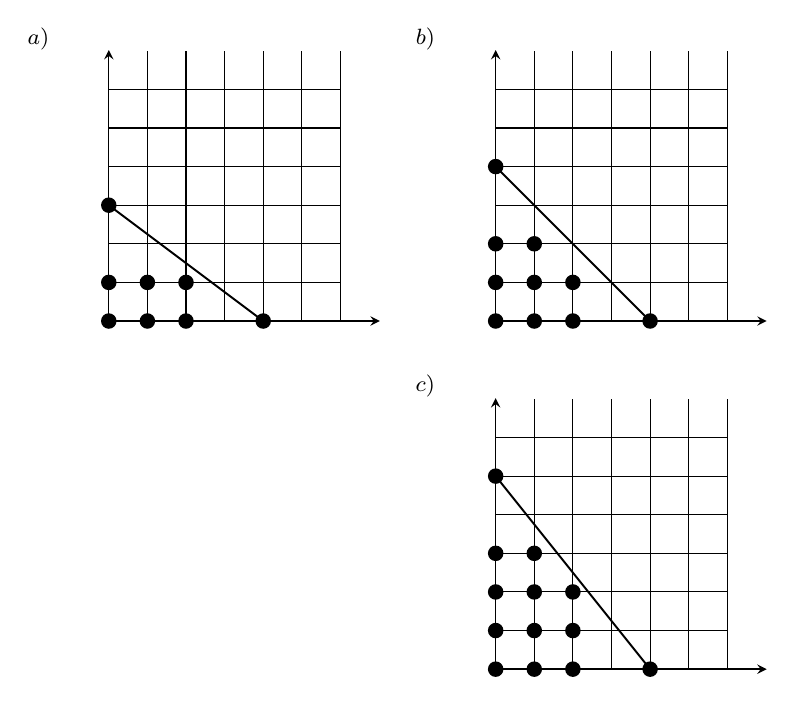
\begin{tikzpicture}[x=1pt,y=1pt,>=stealth,line width=0.5pt]
  \def\u{13.95}
  % ================= panel a) =================
  \begin{scope}[xshift=48.3pt,yshift=134.5pt]
    \draw[line width=0.4pt] \foreach \i in {1,...,6} {(\i*\u,0) -- (\i*\u,{7*\u})};
    \draw[line width=0.4pt] \foreach \j in {1,...,6} {(0,\j*\u) -- ({6*\u},\j*\u)};
    \draw[->] (0,0) -- (0,{7.02*\u});
    \draw[->] (0,0) -- ({7.02*\u},0);
    \draw[line width=0.7pt] (0,{3*\u}) -- ({4*\u},0);
    \foreach \i/\j in {0/0,1/0,2/0,4/0,0/1,1/1,2/1,0/3}
      {\fill ({\i*\u},{\j*\u}) circle[radius=2.8pt];}
  \end{scope}
  % ================= panel b) =================
  \begin{scope}[xshift=188.1pt,yshift=134.5pt]
    \draw[line width=0.4pt] \foreach \i in {1,...,6} {(\i*\u,0) -- (\i*\u,{7*\u})};
    \draw[line width=0.4pt] \foreach \j in {1,...,6} {(0,\j*\u) -- ({6*\u},\j*\u)};
    \draw[->] (0,0) -- (0,{7.02*\u});
    \draw[->] (0,0) -- ({7.02*\u},0);
    \draw[line width=0.7pt] (0,{4*\u}) -- ({4*\u},0);
    \foreach \i/\j in {0/0,1/0,2/0,4/0,0/1,1/1,2/1,0/2,1/2,0/4}
      {\fill ({\i*\u},{\j*\u}) circle[radius=2.8pt];}
  \end{scope}
  % ================= panel c) =================
  \begin{scope}[xshift=188.1pt,yshift=8.7pt]
    \draw[line width=0.4pt] \foreach \i in {1,...,6} {(\i*\u,0) -- (\i*\u,{7*\u})};
    \draw[line width=0.4pt] \foreach \j in {1,...,6} {(0,\j*\u) -- ({6*\u},\j*\u)};
    \draw[->] (0,0) -- (0,{7.02*\u});
    \draw[->] (0,0) -- ({7.02*\u},0);
    \draw[line width=0.7pt] (0,{5*\u}) -- ({4*\u},0);
    \foreach \i/\j in {0/0,1/0,2/0,4/0,0/1,1/1,2/1,0/2,1/2,2/2,0/3,1/3,0/5}
      {\fill ({\i*\u},{\j*\u}) circle[radius=2.8pt];}
  \end{scope}
  % ================= panel labels =================
  \node[inner sep=0pt] at (22.9,236.5) {\fontsize{8}{10}\selectfont$a)$};
  \node[inner sep=0pt] at (162.7,236.5) {\fontsize{8}{10}\selectfont$b)$};
  \node[inner sep=0pt] at (162.7,111.1) {\fontsize{8}{10}\selectfont$c)$};
\end{tikzpicture}

\caption{a）$(A_3,A_2)$ 理论的 Seiberg--Witten 图；b）$(A_3,A_3)$ 理论的 Seiberg--Witten 图；c）$(A_3,A_4)$ 理论的 Seiberg--Witten 图。}
\label{fig:13}
\end{figure}

若相应的非正则奇点具有整数极点，则领头阶系数中还有 $N-2$ 个可以打开的额外参数。这些参数无量纲；幸运的是，谱中确实有 $N-2$ 个维数为二的算子，于是这些无量纲耦合常数自然地与严格边缘（exactly marginal）形变等同起来。与熟悉的 $\sN{=}4$ SYM 理论不同，这些 AD 理论在共形流形上似乎没有弱耦合描述。

有趣的是，把 $x$ 轴与 $y$ 轴互换，算子谱完全相同；因此 $(A_{k-1},A_{N-1})$ 理论与 $(A_{N-1},A_{k-1})$ 理论等价。显式数出库仑分支形变的个数与质量参数的个数，即可证明 $(A_{N-1},A_{k-1})$ 理论电荷格的秩为
\begin{equation}
R = 2n_c+n_f = (k-1)(N-1) .
\label{eq:6.18}\tag{6.18}
\end{equation}
这与 BPS 箭图中箭图节点的个数一致，正如其名字所提示的。

上述事实可用非正则奇点的几何性质来核对。设奇点具有整数极点，阶为 $r=nk/k+2=n+2$，它实际上定义了 $(A_{k-1},A_{nk-1})$ 理论。带这种非正则奇点的模空间维数为
\begin{equation}
d = (n+2)(k^2-k)-2(k^2-1) = (nk-1)(k-1)-(k-1) .
\label{eq:6.19}\tag{6.19}
\end{equation}
这个数等于 $2n_r$，其中 $n_r$ 是库仑分支一般点处规范群的秩；此外还有 $n_f=k-1$ 个质量参数。于是由几何考虑得到电荷格的秩为
\begin{equation}
R = (k-1)(nk-1) ,
\label{eq:6.20}\tag{6.20}
\end{equation}

\subsubsection{Type II SCFT}
\label{sec:6.1.2}

这类 SCFT 由球面上的 type II 非正则奇点定义，SCFT 点处的 Seiberg--Witten 曲线为
\begin{equation}
x^k+z^Nx = 0 ,
\label{eq:6.21}\tag{6.21}
\end{equation}
于是坐标 $x$ 与 $z$ 的标度维数为
\begin{equation}
[x] = \frac{N}{k-1+N},\qquad [z] = \frac{k-1}{k-1+N} .
\label{eq:6.22}\tag{6.22}
\end{equation}
该非正则奇点的极点阶为 $r=N/(k-1)+2$。同样，理论的一般形变完全由相应非正则奇点的牛顿多边形定出。例子见图 \ref{fig:14}。大小为 $k-1$ 的那个 block 与 $(A_{k-2},A_{N-1})$ 理论相同，这一部分的谱分析与 Type I 理论相同。还可以验证，额外的 $x=0$ 线上每个相关算子都有耦合常数与之配对。

\begin{figure}[tbp]
\centering
% Figure 14 -- the Seiberg-Witten curve from the marked integer points
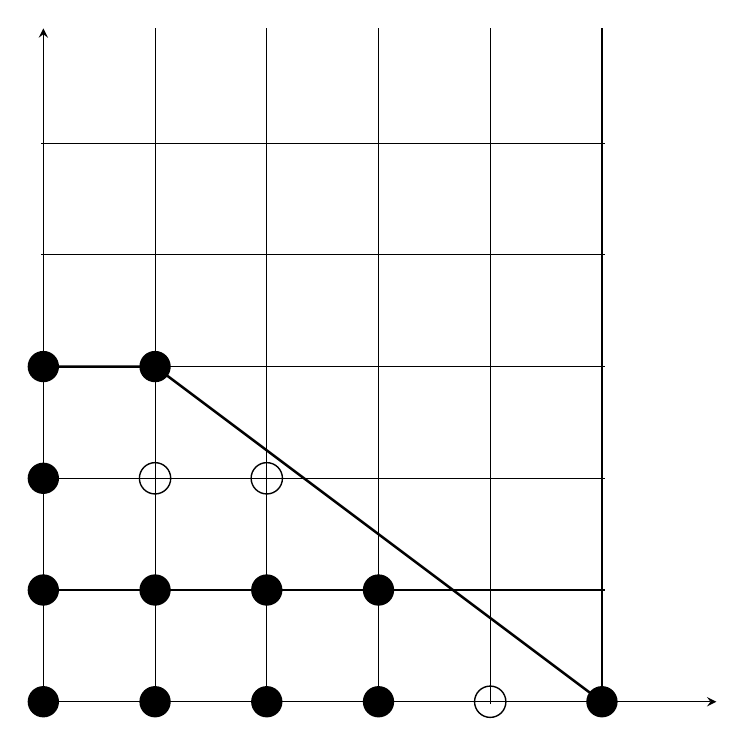
\begin{tikzpicture}[x=1pt,y=1pt,scale=1.08,transform shape,>=stealth,line width=0.5pt]
  \def\u{37.38}
  % ---- grid ----
  \foreach \i in {1,...,5} {\draw[line width=0.4pt] ({24.1+\i*\u},33.5) -- ({24.1+\i*\u},259.6);}
  \foreach \j in {1,...,5} {\draw[line width=0.4pt] (23.4,{34.3+\j*\u}) -- (211.96,{34.3+\j*\u});}
  % ---- axes ----
  \draw[->] (23.4,34.3) -- (249.3,34.3);
  \draw[->] (24.1,33.5) -- (24.1,259.6);
  % ---- Newton polygon ----
  \draw[line width=0.9pt] (24.1,{34.3+3*\u}) -- ({24.1+\u},{34.3+3*\u}) -- ({24.1+5*\u},34.3);
  % ---- marked lattice points ----
  \foreach \i/\j in {0/0,1/0,2/0,3/0,5/0,0/1,1/1,2/1,3/1,0/2,0/3,1/3}
    {\fill ({24.1+\i*\u},{34.3+\j*\u}) circle[radius=5.24pt];}
  \foreach \i/\j in {4/0,1/2,2/2}
    {\draw ({24.1+\i*\u},{34.3+\j*\u}) circle[radius=5.24pt];}
\end{tikzpicture}

\caption{由牛顿多边形所围的带标记整点读出 Seiberg--Witten 曲线。}
\label{fig:14}
\end{figure}

\subsubsection{Type III SCFT}
\label{sec:6.1.3}

用 type III 非正则奇点定义的 SCFT 稍难分析。先看整数极点的情形。此时奇点由一列杨图 $Y_n\subseteq Y_{n-1}\cdots\subseteq Y_1$ 指定，其中 $n=N/k+2$。奇点处的 Seiberg--Witten 曲线为
\begin{equation}
x^k+u_1x^{N-2}+u_2x^{N-3}+\cdots+z^N = 0 ,
\label{eq:6.23}\tag{6.23}
\end{equation}
其中 $u_i$ 经过调节，使根具有 $Y_n$ 所定的退化。形变后的 Seiberg--Witten 曲线与未退化时相同；但并非所有算子都独立，它们之间满足相当复杂的关系。我们想知道谱的标度维数。与正则穿刺点的情形一样，这些信息包含在相应的杨图序列里。一般的 Seiberg--Witten 曲线为
\begin{equation}
x^k+\sum_{i=2}^{k}\Phi_i(z)z^{k-i} = 0 .
\label{eq:6.24}\tag{6.24}
\end{equation}
$\Phi_i$ 中系数为库仑分支算子的 $z$ 最高幂次，由下述数据定出：
\begin{equation}
m_i = \sum_j p_i^{(j)}-2i+1 ,
\label{eq:6.25}\tag{6.25}
\end{equation}
其中 $p_i^{(j)}=i-s_i$，$s_i$ 是第 $j$ 个杨图中第 $i$ 个格子的高度；$\Phi_i$ 具有如下形式
\begin{equation}
\Phi_i = \cdots+u_1z^{m_i-1}+u_2z^{m_i-2}+\cdots+c ,
\label{eq:6.26}\tag{6.26}
\end{equation}
标号为 $u_1$、$u_2$、…、$c$ 的系数就是独立的库仑分支算子。
\typo{原文 p.37 的 (6.25) 与 (5.18) 的 $d_i=\sum_j p_i^{(j)}-2i$ 相差一。两者数的对象不同：(5.18) 数的是第 $i$ 个微分的极点阶，这里数的是 $\Phi_i$ 中库仑分支算子所占的最高 $z$ 幂次，后者比极点阶多一项。两式并不矛盾。}

有两个特例值得再谈，用正则穿刺点定义理论时也会遇到同样情形。第一种是领头阶系数中的数 $m_k$ 为零或负；此时不能再用上述办法求谱，目前我们也找不到系统处理它的方法。另一种是 $m_k$ 非零，但有些别的 $m_j$ 为负；此时仍可用上面的计算求谱，但库仑分支的维数与 Hitchin 纤维化的底的维数不再相等。

若极点阶为分数，可用类似方法求出退化情形的谱。这留给感兴趣的读者。

这些位形并不总能定义 SCFT，因为无量纲耦合（编码在非正则奇点的领头阶矩阵里）与维数为二的算子之间可能没有配对。判断何时才能成为 SCFT，留待以后研究。

\subsubsection{再加一个正则奇点：Type IV SCFT}
\label{sec:6.1.4}

可以在上述情形上再加一个正则奇点，并在红外找到 AD 理论。图 \ref{fig:15} 给出一个例子。注意，这里把非正则奇点所有可能的形变都打开，好让来自正则奇点的相关形变能有耦合常数与之配对。于是先前不允许的那些耦合常数在此起了重要作用。

计算 Seiberg--Witten 曲线时，用到正则穿刺点杨图 $Y_0$ 中的数据。例如，由正则奇点带来的独立库仑分支参数在 Seiberg--Witten 曲线中具有如下形式
\begin{equation}
\Phi_i = \cdots+\bigl(v_1z^{-1}+\cdots+v_{n_i}z^{-n_i}\bigr) ,
\label{eq:6.27}\tag{6.27}
\end{equation}
这里 $\Phi_i$ 是 $i$ 次微分；$n_i=i-s_i$，其中 $s_i$ 是杨图 $Y_0$ 中第 $i$ 个格子的高度。
\typo{原文 p.38 在此处措辞自我重复（「$i$ the $i$th box」与「$s_i$ the height of the $i$th box」连用），译文按「$s_i$ 是第 $i$ 个格子的高度」处理。}

\begin{figure}[tbp]
\centering
% Figure 15 -- Seiberg-Witten graph for an irregular + a regular singularity
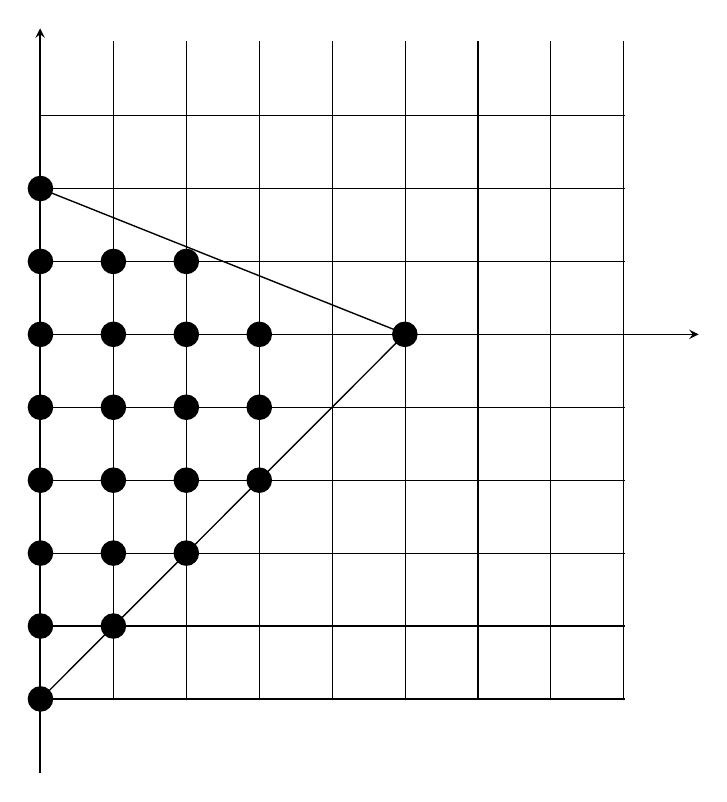
\begin{tikzpicture}[x=1pt,y=1pt,scale=1.05,transform shape,>=stealth,line width=0.5pt]
  \def\u{25.095}
  % ---- grid ----
  \foreach \i in {0,...,8} {\draw[line width=0.4pt] (66.5,28.4) ++(\i*\u,0) -- ++(0,227.1);}
  \foreach \j in {-5,...,3} {\draw[line width=0.4pt] (65.9,{154.4+\j*\u}) -- (267.8,{154.4+\j*\u});}
  % ---- axes ----
  \draw[->] (65.9,154.4) -- (293,154.4);
  \draw[->] (66.4,3.4) -- (66.4,259.7);
  % ---- the two Newton-polygon edges ----
  \draw (66.6,28.9) -- (191.9,154.4);
  \draw (65.9,204.8) -- (192.6,154.3);
  % ---- marked points ----
  \foreach \j in {2,1,0,-1,-2,-3,-4,-5} {\fill (66.5,{154.4+\j*\u}) circle[radius=4.4pt];}
  \foreach \j in {1,0,-1,-2,-3,-4}     {\fill (91.6,{154.4+\j*\u}) circle[radius=4.4pt];}
  \foreach \j in {1,0,-1,-2,-3}        {\fill (116.7,{154.4+\j*\u}) circle[radius=4.4pt];}
  \foreach \j in {0,-1,-2}             {\fill (141.8,{154.4+\j*\u}) circle[radius=4.4pt];}
  \fill (191.9,154.4) circle[radius=4.4pt];
\end{tikzpicture}

\caption{带一个非正则奇点与一个正则奇点的理论的 Seiberg--Witten 图。}
\label{fig:15}
\end{figure}

正则穿刺点可以带有非阿贝尔味对称性，这类 SCFT 在构造渐近自由理论时很重要。在球上放多个非正则奇点所定义的理论里，它们会自然出现：相应的四维理论是把这些 AD 理论一起规范化得到的渐近自由理论，而非正则奇点总位于退化极限下的边界上。

\subsection{三维镜像对称}
\label{sec:6.2}

三维镜像理论同样可以通过寻找接在非正则奇点上的箭图得到。目前只知道整数极点非正则奇点所定义的理论的三维镜像；这类奇点由一列杨图 $Y_n\subseteq Y_{n-1}\cdots\subseteq Y_1$ 分类，其中 $Y_j$ 由 $Y_{j+1}$ 的每一列进一步分拆得到。相应的数学考虑见文献 \cite{39}，其结果的解释正是 Argyres--Douglas 理论的三维镜像对称。

\routenote{原文 pp.38--39。镜像箭图分三步造出。先把 $Y_n$ 的每一列变成一个节点，节点之间按极点阶的整数部分放箭；再沿 $Y_{n-1},\dots,Y_2$ 逐层细分节点；最后把 $Y_1$ 这一层换成正则奇点处早已熟悉的箭图支链。三步拼起来，箭图节点的总秩恰为 $k$。}

三维镜像理论按如下步骤逐步构造。设 $Y_n$ 的分拆为 $[n_1,n_2,\dots,n_r]$，第一步的箭图有 $r$ 个节点，每个节点的秩为 $n_i$，即 $U(n_i)$ 的秩；各节点之间还有 $n-2$ 支箭，代表双基本表示，第一步见图 \ref{fig:16}。第二步：设 $Y_1$ 中某个 $n_i$ 在杨图 $Y_{n-1}$ 中进一步分拆为 $[m_{i1},m_{i2},\dots,m_{is}]$。于是把第一步中秩为 $n_i$ 的箭图节点分裂为 $s$ 个箭图节点，新节点的秩由分拆 $m_{ij}$ 定出，这些新节点之间放 $n-3$ 支箭。此外，分裂出的节点与其他簇中的节点之间仍保留 $n-2$ 支箭，见图 \ref{fig:16}。对每个杨图都做同样的分裂，直到 $Y_2$，就得到由若干节点与箭组成的箭图。注意，所有箭图节点的秩之和为 $k$。

\typo{原文 p.39 此句写「设 $Y_1$ 中某个 $n_i$ 在杨图 $Y_{n-1}$ 中进一步分拆为」。第一步分拆的对象是 $Y_n$，而 $Y_{n-1}$ 是把 $Y_n$ 的每一列进一步分拆得到的（见 Case 1 的定义），故这里应为 $Y_n$；$Y_1$ 是这条链的最后一项，对应质量矩阵，下一段才用到。译文照录原文的 $Y_1$。}

$Y_1$ 即质量矩阵这一层需要特殊处理：若 $Y_2$ 的某一列高为 $l$，而它在 $Y_1$ 中进一步分拆为 $[l_1,l_2,\dots,l_t]$，则不按上述方式分解这个节点，而是像正则奇点那样接一条箭图支链（quiver leg/tail），其总格数为 $l$ \cite{38}。具体地说，定义 $h_i=\sum_{j=t-i+1}^{t}l_j$，这一部分的箭图支链见图 \ref{fig:16}。

若另有一个由杨图指定的正则奇点，则先按图 \ref{fig:16} 底部所示接一条箭图支链，总格数为 $k$。然后把 $U(k)$ 节点按非正则奇点的杨图 $Y_2$ 所定的模式 spray。最后把两个箭图粘合起来，做法是把正则奇点支链上经 spray 得到的节点与非正则奇点箭图中的节点认同。

\begin{figure}[tbp]
\centering
% Figure 16 -- step 1 / step 2 quivers and the quiver tail of the regular singularity
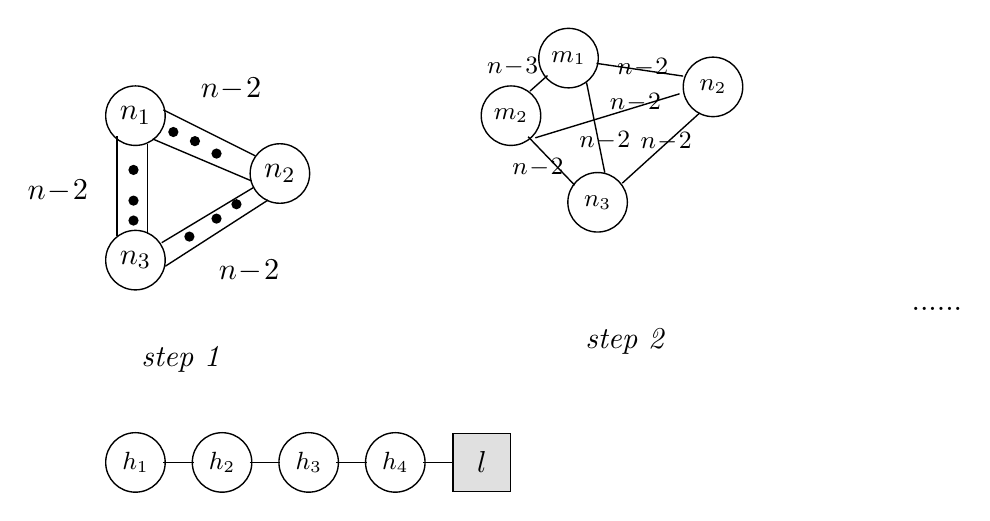
\begin{tikzpicture}[x=1pt,y=1pt,>=stealth,line width=0.5pt,
   circ/.style={circle,draw,minimum size=21.5pt,inner sep=0pt}]
  \def\rr{1.85}
  % ======================== step 1 ========================
  % --- n1--n3 ribbon ---
  \draw (50.1,104.0) -- (50.1,140.1);
  \draw (61.2,105.0) -- (61.2,137.5);
  \foreach \y in {384.0,395.1,402.3} {\fill (56.1,{512-\y}) circle[radius=\rr pt];}
  % --- n1--n2 ribbon ---
  \draw (63.0,139.2) -- (98.8,124.0);
  \draw (66.9,149.7) -- (100.1,133.1);
  \fill (70.5,141.7) circle[radius=\rr pt];
  \fill (78.3,138.4) circle[radius=\rr pt];
  \fill (86.1,133.9) circle[radius=\rr pt];
  % --- n3--n2 ribbon ---
  \draw (66.3,101.7) -- (99.4,121.6);
  \draw (67.6,93.2) -- (104.7,117.1);
  \fill (76.3,103.9) circle[radius=\rr pt];
  \fill (86.1,110.4) circle[radius=\rr pt];
  \fill (93.3,115.6) circle[radius=\rr pt];
  % ======================== step 2 ========================
  \draw (199.4,156.5) -- (205.7,162.1);
  \draw (223.4,166.5) -- (254.7,161.9);
  \draw (219.8,159.6) -- (226.4,127.0);
  \draw (198.7,140.0) -- (215.5,122.5);
  \draw (201.3,139.6) -- (253.4,155.5);
  \draw (232.7,123.2) -- (260.5,148.4);
  % ======================== nodes ========================
  \node[circ] (n1) at (56.8,147.6)   {\fontsize{11}{13}\selectfont$n_1$};
  \node[circ] (n2) at (109.0,126.7)  {\fontsize{11}{13}\selectfont$n_2$};
  \node[circ] (n3) at (56.8,95.4)    {\fontsize{11}{13}\selectfont$n_3$};
  \node[circ] (mm1) at (213.3,168.4) {\fontsize{9}{11}\selectfont$m_1$};
  \node[circ] (mm2) at (192.5,147.6) {\fontsize{9}{11}\selectfont$m_2$};
  \node[circ] (sn3) at (223.8,116.3) {\fontsize{9}{11}\selectfont$n_3$};
  \node[circ] (sn2) at (265.5,158.0) {\fontsize{9}{11}\selectfont$n_2$};
  % ======================== quiver tail ========================
  \draw (66.8,22.3) -- (77.9,22.3);
  \draw (98.1,22.3) -- (109.2,22.3);
  \draw (129.4,22.3) -- (140.5,22.3);
  \draw (160.8,22.3) -- (171.6,22.3);
  \draw[fill=black!12] (171.6,11.9) rectangle (192.4,32.8);
  \node[circ] (h1) at (56.8,22.3)  {\fontsize{9}{11}\selectfont$h_1$};
  \node[circ] (h2) at (88.1,22.3)  {\fontsize{9}{11}\selectfont$h_2$};
  \node[circ] (h3) at (119.4,22.3) {\fontsize{9}{11}\selectfont$h_3$};
  \node[circ] (h4) at (150.7,22.3) {\fontsize{9}{11}\selectfont$h_4$};
  \node[inner sep=0pt] at (182.0,22.35) {\fontsize{11}{13}\selectfont$l$};
  % ======================== labels ========================
  \node[inner sep=0pt] at (91.35,157.35) {\fontsize{11}{13}\selectfont$n\!-\!2$};
  \node[inner sep=0pt] at (97.85,91.55)  {\fontsize{11}{13}\selectfont$n\!-\!2$};
  \node[inner sep=0pt] at (28.75,120.25) {\fontsize{11}{13}\selectfont$n\!-\!2$};
  \node[inner sep=0pt] at (193.1,165.5)  {\fontsize{9}{11}\selectfont$n\!-\!3$};
  \node[inner sep=0pt] at (240.1,164.85) {\fontsize{9}{11}\selectfont$n\!-\!2$};
  \node[inner sep=0pt] at (237.45,152.45){\fontsize{9}{11}\selectfont$n\!-\!2$};
  \node[inner sep=0pt] at (226.4,138.75) {\fontsize{9}{11}\selectfont$n\!-\!2$};
  \node[inner sep=0pt] at (248.55,138.1) {\fontsize{9}{11}\selectfont$n\!-\!2$};
  \node[inner sep=0pt] at (202.25,129.0) {\fontsize{9}{11}\selectfont$n\!-\!2$};
  \node[inner sep=0pt] at (73.1,59.55)   {\fontsize{11}{13}\itshape step 1};
  \node[inner sep=0pt] at (233.55,66.05) {\fontsize{11}{13}\itshape step 2};
  \node[inner sep=0pt] at (346.4,77.85)  {\fontsize{11}{13}\selectfont......};
\end{tikzpicture}

\caption{第一步：若第一个杨图 $Y_n$ 的分拆为 $[n_1,n_2,n_3]$，则有一条含三个节点的箭图支链，各节点的秩为 $n_i$，这些节点之间有 $n-2$ 支箭。第二步：若 $n_1$ 在 $Y_{n-1}$ 中进一步分拆为 $[m_1,m_2]$，则把秩为 $n_1$ 的箭图节点分裂为两个箭图节点，秩分别为 $m_1$ 与 $m_2$；$m_i$ 与 $n_1$、$n_2$ 之间的箭不变，$m_1$ 与 $m_2$ 之间新添 $n-3$ 支箭。对其他杨图重复同样步骤，直到 $Y_2$ 为止。底部：若 $Y_2$ 中高为 $l$ 的列进一步分拆为 $[l_1,l_2,\dots,l_t]$，则在 $(Y_n,\dots,Y_2)$ 所定箭图中秩为 $l$ 的节点上接一条箭图支链。}
\label{fig:16}
\end{figure}

下面给出几个显例。

例 1：有一个极点阶为三的非正则奇点，其杨图为 $[2,2]$、$[1,1,1,1]$、$[1,1,1,1]$，箭图见图 \ref{fig:17}a。

例 2：有一个极点阶为四的非正则奇点，其杨图为 $[3,2]$、$[3,1,1]$、$[3,1,1]$、$[1,1,1,1,1]$，箭图见图 \ref{fig:17}b。

例 3：有一个极点阶为三的非正则奇点，其杨图为 $[1,1,1,1]$、$[1,1,1,1]$、$[1,1,1,1]$，另有一个满正则奇点，箭图见图 \ref{fig:17}c。

\begin{figure}[tbp]
\centering
% Figure 17 -- 3d mirrors for the AD theories of Examples 1, 2, 3
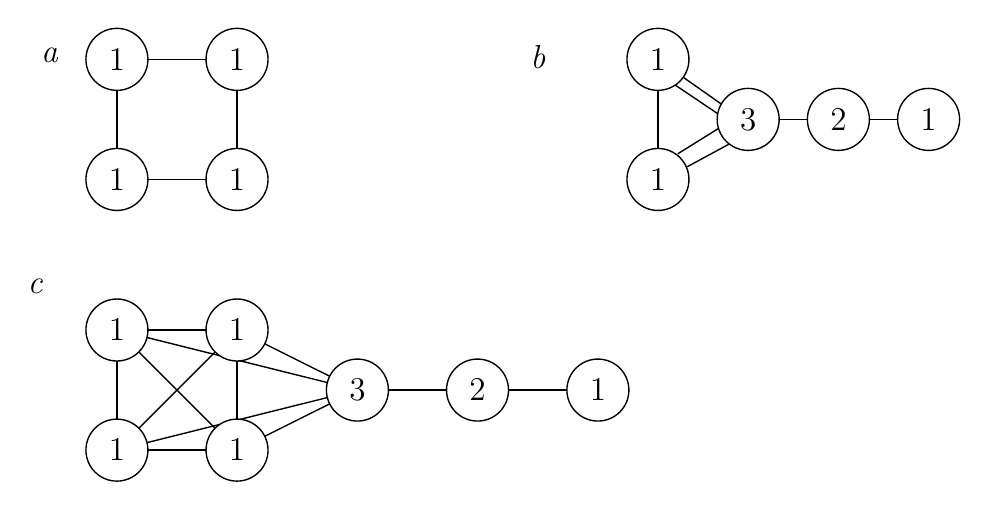
\begin{tikzpicture}[x=1pt,y=1pt,>=stealth,line width=0.5pt,
   nd/.style={circle,draw,fill=white,minimum size=22.4pt,inner sep=0pt}]
  % ===================== a) =====================
  \draw (37.6,164.0) rectangle (81.0,120.6);
  % ===================== b) =====================
  \draw (233.1,164.0) -- (233.1,120.6);
  \draw (238.3,155.4) -- (255.1,144.1);
  \draw (242.4,157.4) -- (256.5,147.5);
  \draw (240.3,129.9) -- (255.1,139.1);
  \draw (243.7,125.2) -- (259.2,133.6);
  \draw (265.7,142.3) -- (298.3,142.3) -- (330.9,142.3);
  % ===================== c) =====================
  \draw (37.6,66.2) -- (81.0,66.2) -- (81.0,22.8) -- (37.6,22.8) -- cycle;
  \draw (37.6,66.2) -- (81.0,22.8);
  \draw (37.6,22.8) -- (81.0,66.2);
  \draw (37.6,66.2) -- (124.5,44.5);
  \draw (81.0,66.2) -- (124.5,44.5);
  \draw (37.6,22.8) -- (124.5,44.5);
  \draw (81.0,22.8) -- (124.5,44.5);
  \draw (124.5,44.5) -- (167.9,44.5) -- (211.4,44.5);
  % ===================== nodes =====================
  \foreach \x/\y in {37.6/164.0,81.0/164.0,81.0/120.6,37.6/120.6}
    {\node[nd] at (\x,\y) {\fontsize{12}{14}\selectfont 1};}
  \foreach \x/\y in {233.1/164.0,233.1/120.6}
    {\node[nd] at (\x,\y) {\fontsize{12}{14}\selectfont 1};}
  \node[nd] at (265.7,142.3) {\fontsize{12}{14}\selectfont 3};
  \node[nd] at (298.3,142.3) {\fontsize{12}{14}\selectfont 2};
  \node[nd] at (330.9,142.3) {\fontsize{12}{14}\selectfont 1};
  \foreach \x/\y in {37.6/66.2,81.0/66.2,37.6/22.8,81.0/22.8}
    {\node[nd] at (\x,\y) {\fontsize{12}{14}\selectfont 1};}
  \node[nd] at (124.5,44.5) {\fontsize{12}{14}\selectfont 3};
  \node[nd] at (167.9,44.5) {\fontsize{12}{14}\selectfont 2};
  \node[nd] at (211.4,44.5) {\fontsize{12}{14}\selectfont 1};
  % ===================== panel letters =====================
  \node[inner sep=0pt] at (13.1,165.45) {\fontsize{12}{14}\itshape a};
  \node[inner sep=0pt] at (189.7,164.75) {\fontsize{12}{14}\itshape b};
  \node[inner sep=0pt] at (8.05,81.9)   {\fontsize{12}{14}\itshape c};
\end{tikzpicture}

\caption{例 1、例 2、例 3 所述 AD 理论的三维镜像。}
\label{fig:17}
\end{figure}

\subsection{SCFT 之间的等价}
\label{sec:6.3}

（a）我们已经说明 $(A_{k-1},A_{N-1})$ 理论与 $(A_{N-1},A_{k-1})$ 理论相同。Type II 与 Type IV 理论之间还有另一个同构。考虑带一个单正则奇点的 Type IV 理论，其中的非正则奇点就是定义 $(A_{k-1},A_{N-1})$ 理论的那一个；这里需要 $N\ge k$。一个例子见图 \ref{fig:18}a。$[x]$ 与 $[z]$ 的标度维数仍为
\begin{equation}
[x] = \frac{N}{N+k},\qquad [z] = \frac{k}{N+k} .
\label{eq:6.28}\tag{6.28}
\end{equation}
正则穿刺点还带来一个额外的质量参数，而多出来的 $k-1$ 个库仑分支算子的维数为
\begin{equation}
u_i = [z]+i[x],\qquad 2\le i\le k .
\label{eq:6.29}\tag{6.29}
\end{equation}
\typo{原文 p.40 的 (6.29) 与 (6.31) 都把算子名直接写成标度维的组合，左边的维数括号被省掉了。按上一句「多出来的 $k-1$ 个库仑分支算子的维数为」，这里应读作 $[u_i]=[z]+i[x]$、$[v_i]=[x']+i[z']$。译文照录。}

现在看由图 \ref{fig:18}b 给出的 Type II 理论，它由六维 $A_N$ 理论实现。牛顿多边形的三角形部分与 $(A_{N-1},A_{k-1})$ 理论相同，而后者等价于 $(A_{k-1},A_{N-1})$ 理论。其标度维数为
\begin{equation}
[x'] = \frac{k}{N+k},\qquad [z'] = \frac{N}{N+k} .
\label{eq:6.30}\tag{6.30}
\end{equation}
只需再求出 $x=0$ 线上额外算子的标度维数，它们形如
\begin{equation}
v_i = [x']+i[z'],\qquad 0\le i\le k .
\label{eq:6.31}\tag{6.31}
\end{equation}
于是 $v_0$ 是耦合常数，$v_1$ 是质量参数。注意 $[x]$ 与 $[z']$ 的标度维数相同，因此库仑分支谱与上面的实现完全相同。这个同构通过交换 $x$ 与 $z$ 坐标实现，而这也正是 $(A,A)$ 理论同构的机制。

\begin{figure}[tbp]
\centering
% Figure 18 -- a) Type IV SCFT Newton polygon, b) Type II SCFT Newton polygon
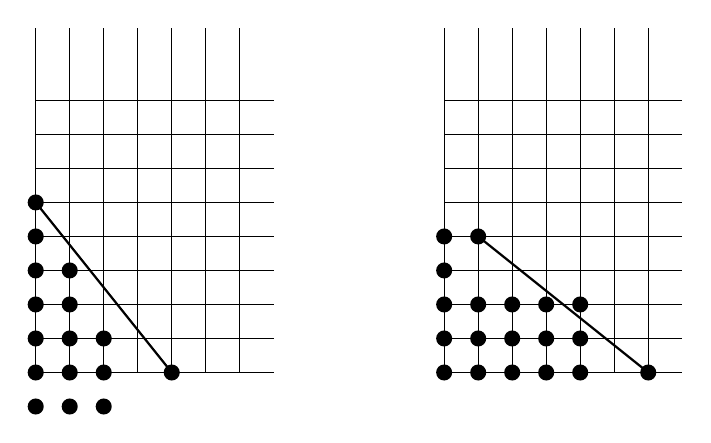
\begin{tikzpicture}[x=1pt,y=1pt,>=stealth,line width=0.5pt]
  \def\u{12.29}
  % ===================== panel a) =====================
  \foreach \i in {0,...,6} {\draw[line width=0.4pt] ({\i*\u},0) -- ({\i*\u},124.4);}
  \foreach \j in {0,...,8} {\draw[line width=0.4pt] (0,{\j*\u}) -- ({7*\u},{\j*\u});}
  \draw[line width=0.8pt] (0,{5*\u}) -- ({4*\u},0);
  \foreach \i/\j in {0/5,0/4,0/3,1/3,0/2,1/2,0/1,1/1,2/1,0/0,1/0,2/0,4/0,0/-1,1/-1,2/-1}
    {\fill ({\i*\u},{\j*\u}) circle[radius=2.9pt];}
  % ===================== panel b) =====================
  \begin{scope}[xshift=147.6pt]
    \foreach \i in {0,...,6} {\draw[line width=0.4pt] ({\i*\u},0) -- ({\i*\u},124.4);}
    \foreach \j in {0,...,8} {\draw[line width=0.4pt] (0,{\j*\u}) -- ({7*\u},{\j*\u});}
    \draw[line width=0.8pt] ({\u},{4*\u}) -- ({6*\u},0);
    \foreach \i/\j in {0/4,1/4,0/3,0/2,1/2,2/2,3/2,4/2,0/1,1/1,2/1,3/1,4/1,0/0,1/0,2/0,3/0,4/0,6/0}
      {\fill ({\i*\u},{\j*\u}) circle[radius=2.9pt];}
  \end{scope}
\end{tikzpicture}

\caption{a）由六维 $A_3$ 理论定义的 Type IV SCFT：非正则奇点的形式由牛顿多边形给出，此外还有一个单正则奇点；图中只写出正则奇点给出的库仑分支参数。b）由 $A_5$ 理论以适当的非正则奇点定义的 Type II SCFT；显式算出谱之后可知，这个理论与 a）等价。}
\label{fig:18}
\end{figure}

再对 $k=2$ 稍作评论：用正则奇点的第一种实现，就是熟悉的 $(A_1,D_{N+2})$ 理论，它由六维 $A_1$ 理论给出。下面说明，这类理论也能只用 $A_N$ 理论的一个非正则奇点实现。

还有更多类似的同构，感兴趣的读者可以自己找一找，这件事颇有乐趣。

\subsubsection{class S 理论的非正则实现}
\label{sec:6.3.1}

\routenote{原文 pp.40--42。这里的路线是把三维镜像反过来用：同一个镜像箭图可以有多种「切成块」的读法，每块读法对应一种奇点结构，于是同一个 class S 理论得到多种非正则实现。作者的检验依据是镜像相同，故库仑分支维数、希格斯分支维数与味对称性都相同。}

还有一类可能的同构，来自对三维镜像对称的考察。最令人惊讶的发现或许是：用带正则穿刺点的球定义的所有理论，都能用非正则奇点实现；而且实现并不唯一。先较仔细地研究带四个味的 $\SU(2)$ 理论，稍后再给一般情形。这个理论有 Gaiotto 找到的六维构造：$A_1$ 理论在球面上放四个正则穿刺点。它的三维镜像很简单，见图 \ref{fig:19}a。

同一个理论有许多非正则实现。先看秩为三的实现：按图 \ref{fig:19}b 的方式看三维镜像。这种看法意味着有一个满正则穿刺点，以及一个带两个满杨图的非正则穿刺点。若按图 \ref{fig:19}c 排布镜像，就得到秩为四的实现：一个分拆为 $[2,2]$ 的正则奇点，加一个带两个满杨图的非正则奇点。秩为五的实现由按图 \ref{fig:19}d 分解镜像得到：只有一个非正则奇点，它有三个杨图，分拆为 $Y_3=[3,2]$、$Y_2=[2,1,1,1]$、$Y_3=[1,1,1,1,1]$。最后还有秩为六的实现：唯一的非正则奇点分拆为 $Y_3=[4,2]$、$Y_2=[2,1,1,1,1]$、$Y_3=[2,1,1,1,1]$，其三维镜像的分解见图 \ref{fig:19}e。
\typo{原文 p.42 在秩 5 与秩 6 的实现中把 $Y_3$ 写了两遍（如 $Y_3=[3,2]$、$Y_2=[2,1,1,1]$、$Y_3=[1,1,1,1,1]$），第三个杨图应为 $Y_1$。译文照录。}

\begin{figure}[tbp]
\centering
% Figure 19 -- a)-e) different decompositions of the 3d mirror of SU(2) with four flavours
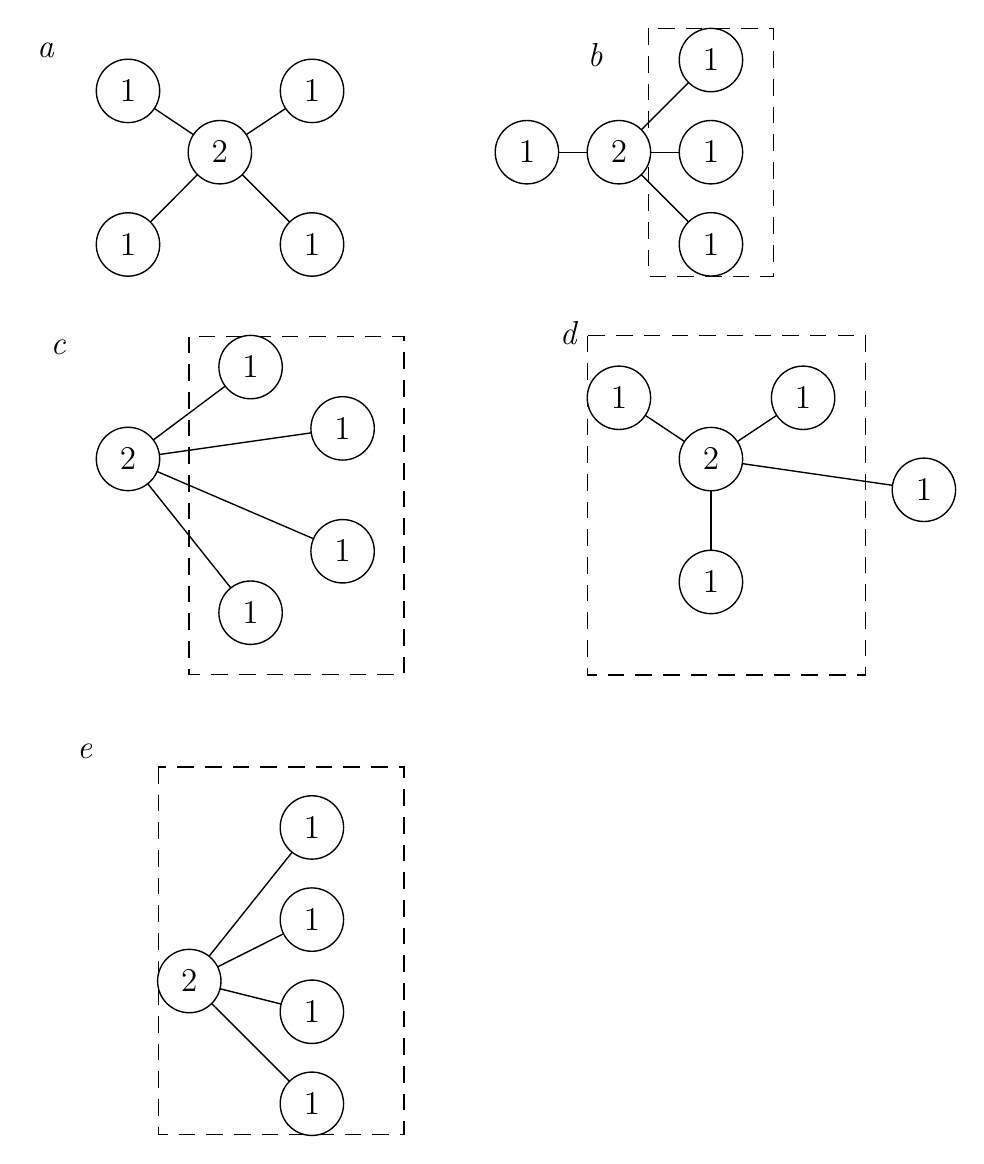
\begin{tikzpicture}[x=1pt,y=1pt,>=stealth,line width=0.5pt,
   nd/.style={circle,draw,fill=white,minimum size=22.9pt,inner sep=0pt,
              font=\fontsize{12}{12}\selectfont},
   bx/.style={draw,line width=0.5pt,dash pattern=on 6pt off 4pt}]
  % ---------------- a) ----------------
  \draw (41.5,381.8) -- (74.7,359.65);
  \draw (41.5,326.3) -- (74.7,359.65);
  \draw (74.7,359.65) -- (108.0,381.8);
  \draw (74.7,359.65) -- (108.0,326.3);
  \node[nd] at (74.7,359.65) {2};
  \node[nd] at (41.5,381.8) {1};
  \node[nd] at (41.5,326.3) {1};
  \node[nd] at (108.0,381.8) {1};
  \node[nd] at (108.0,326.3) {1};
  \node[anchor=base west,font=\fontsize{12.5}{15}\selectfont\itshape] at (5,394) {a};
  % ---------------- b) ----------------
  \draw[bx] (229.6,404.4) rectangle (274.7,314.8);
  \draw (185.65,359.65) -- (218.9,359.65);
  \draw (218.9,359.65) -- (252.15,359.65);
  \draw (218.9,359.65) -- (252.15,392.95);
  \draw (218.9,359.65) -- (252.15,326.35);
  \node[nd] at (185.65,359.65) {1};
  \node[nd] at (218.9,359.65) {2};
  \node[nd] at (252.15,359.65) {1};
  \node[nd] at (252.15,392.95) {1};
  \node[nd] at (252.15,326.35) {1};
  \node[anchor=base west,font=\fontsize{12.5}{15}\selectfont\itshape] at (204,390.5) {b};
  % ---------------- c) ----------------
  \draw[bx] (63.6,293.0) rectangle (141.3,171.0);
  \draw (41.5,248.8) -- (85.8,282.0);
  \draw (41.5,248.8) -- (119.05,259.85);
  \draw (41.5,248.8) -- (119.05,215.45);
  \draw (41.5,248.8) -- (85.8,193.25);
  \node[nd] at (41.5,248.8) {2};
  \node[nd] at (85.8,282.0) {1};
  \node[nd] at (119.05,259.85) {1};
  \node[nd] at (119.05,215.45) {1};
  \node[nd] at (85.8,193.25) {1};
  \node[anchor=base west,font=\fontsize{12.5}{15}\selectfont\itshape] at (10,286.5) {c};
  % ---------------- d) ----------------
  \draw[bx] (207.5,293.4) rectangle (308.0,170.7);
  \draw (252.15,248.75) -- (218.9,270.9);
  \draw (252.15,248.75) -- (285.45,270.9);
  \draw (252.15,248.75) -- (252.15,204.35);
  \draw (252.15,248.75) -- (329.1,237.65);
  \node[nd] at (252.15,248.75) {2};
  \node[nd] at (218.9,270.9) {1};
  \node[nd] at (285.45,270.9) {1};
  \node[nd] at (252.15,204.35) {1};
  \node[nd] at (329.1,237.65) {1};
  \node[anchor=base west,font=\fontsize{12.5}{15}\selectfont\itshape] at (194,290) {d};
  % ---------------- e) ----------------
  \draw[bx] (52.5,137.5) rectangle (141.2,4.8);
  \draw (63.65,60.15) -- (107.95,115.65);
  \draw (63.65,60.15) -- (107.95,82.35);
  \draw (63.65,60.15) -- (107.95,49.05);
  \draw (63.65,60.15) -- (107.95,15.8);
  \node[nd] at (63.65,60.15) {2};
  \node[nd] at (107.95,115.65) {1};
  \node[nd] at (107.95,82.35) {1};
  \node[nd] at (107.95,49.05) {1};
  \node[nd] at (107.95,15.8) {1};
  \node[anchor=base west,font=\fontsize{12.5}{15}\selectfont\itshape] at (19.5,140.5) {e};
\end{tikzpicture}

\caption{带四个味的 $\SU(2)$ 理论的三维镜像的不同分解。每种分解对应一种奇点结构的组合。a）球上有四个正则奇点，每个带一条 $1-2$ 的箭图支链，把各处的 $U(2)$ 味对称性粘合起来即得三维镜像。b）这是秩为三的实现，有一个带箭图支链 $1-2-3$ 的正则奇点，而秩为二的非正则奇点给出一个含三个孤立 $U(1)$ 节点的箭图。于是把正则奇点箭图的 $U(3)$ 节点 spray 成三个 $U(1)$ 节点，再与非正则奇点的箭图粘合。c）这是秩为四的实现，正则奇点的杨图为 $[2,2]$，再加上极点阶为二的非正则奇点，其箭图含四个孤立节点。d）秩为五的实现，只有一个非正则奇点。e）秩为六的实现，只有一个非正则奇点。}
\label{fig:19}
\end{figure}

事实上还有另一种非正则奇点构造，它的三维镜像尚不知道。我们的发现基于线性箭图 $\SU(2)-\SU(4)$，其中 $\SU(4)$ 群并非共形。文献 \cite{32} 指出，其六维构造需要黎曼球上有两个非正则奇点，而 $\SU(2)-4$ 这条支链由如下结构的非正则奇点描述
\begin{equation}
\Phi = z^{-1-\frac{1}{2}}\diag(1,\ w,\ -1,\ -w) ,
\label{eq:6.32}\tag{6.32}
\end{equation}
外加一个 $\SU(4)$ 满正则奇点。我们猜想，这是带四个味的 $\SU(2)$ 理论的另一个秩为四的实现。

把上述做法推广到球面上定义的任何 class S 理论并不难。三维镜像不过是一个星形箭图，它由来自各个穿刺点的箭图支链粘合而成。同一个三维镜像箭图还可以有别的看法，而这些看法都能用非正则奇点实现。不过，不同的实现确实很多。

有几项显式的检验可做：既然三维镜像相同，库仑分支维数与希格斯分支维数就相同，味对称性也相同。这些证据强烈表明：用非正则奇点定义的理论，与球面上带正则奇点定义的 class S 理论是同一个理论。此外，只要取若干有量纲参数之间的比值，就能凑出足够多的无量纲规范耦合常数。我们认为这个值得注意的对偶性很重要，将来还要进一步研究。

\subsection{关于 $R(B)$ 与中心荷 $a$、$c$ 的猜想}
\label{sec:6.4}

中心荷的计算与 $A_1$、$A_2$ 理论的做法很相似：先用镜像对称与算子谱的标度维数算出一部分理论的中心荷，再把结果代入公式 (2.8) 得到函数 $R(B)$。最后用 $R(B)$ 算出这一类中其他理论的中心荷。我们假定 $R(B)$ 有统一的公式，并对 $(A_{k-1},A_{N-1})$ 理论给出显式形式。猜想依据的是下面 $A_1$、$A_2$ 的已知公式，以及 $k$ 与 $N$ 交换下的不变性。我们此前对 $A_1$、$A_2$ 理论的计算给出
\begin{equation}
A_1:\quad R(B) = \frac{1}{2}\,\frac{N(N-1)}{N+2} .
\label{eq:6.33}\tag{6.33}
\end{equation}
\begin{equation}
A_2:\quad R(B) = \frac{3}{2}\,\frac{N(N-1)}{N+3} .
\label{eq:6.34}\tag{6.34}
\end{equation}

我们猜想的普遍公式为
\begin{equation}
A_{k-1}:\quad R(B) = \frac{k(k-1)}{4}\,\frac{N(N-1)}{N+k} ,
\label{eq:6.35}\tag{6.35}
\end{equation}
它在交换 $k$ 与 $N$ 下不变，并能回到 $A_1$、$A_2$ 的情形。

\subsubsection{来自镜像对称的验证}
\label{sec:6.4.1}

可以用三维镜像来检验这个猜想。取三维镜像已知的 $(A_{k-1},A_{nk-1})$ 理论。先用上面猜想的 $R(B)$ 形式算它的中心荷。Seiberg--Witten 曲线为
\begin{equation}
x^k+\bigl(u_1z^{2n-1}+\cdots+u_{2n}\bigr)x^{k-2}
+\bigl(v_1z^{3n-1}+\cdots+v_{3n}\bigr)x^{k-3}
+\cdots+\bigl(z^{nk}+\cdots+c_{nk}\bigr) = 0 ,
\label{eq:6.36}\tag{6.36}
\end{equation}
于是 $z$ 的标度维数为 $[z]=1/(n+1)$。$R(A)$ 可由谱的标度维数求出：
\begin{equation}
R(A) = \sum\bigl(D(u_i)-1\bigr)
= \frac{3kn-3k^2n+kn^2-3k^2n^2+2k^3n^2}{12(1+n)} ,
\label{eq:6.37}\tag{6.37}
\end{equation}
而 $R(B)$ 由我们的拟设给出：
\begin{equation}
R(B) = \frac{k(k-1)}{4}\,\frac{n(nk-1)}{n+1} .
\label{eq:6.38}\tag{6.38}
\end{equation}
利用公式 (2.8)，中心荷为
\begin{equation}
c = \frac{(-1+k)(-2-2n+kn^2+k^2n^2)}{12(1+n)},\qquad
a = \frac{(-1+k)(-5-5n+2kn^2+2k^2n^2)}{24(1+n)} .
\label{eq:6.39}\tag{6.39}
\end{equation}

现在改用另一组方程与三维镜像对称来算。三维镜像理论的库仑分支维数为 $k-1$，因此
\begin{equation}
2a-c = \frac{1}{4}\sum_{i=1}^{r}\bigl(2D(u_i)-1\bigr)
= \frac{3-3k+3n-3kn-kn^2+k^3n^2}{12(1+n)},\qquad
a-c = -\frac{k-1}{24} .
\label{eq:6.40}\tag{6.40}
\end{equation}
我们又得到
\begin{equation}
a = \frac{(-1+k)(-5-5n+2kn^2+2k^2n^2)}{24(1+n)},\qquad
c = \frac{(-1+k)(-2-2n+kn^2+k^2n^2)}{12(1+n)} ,
\label{eq:6.41}\tag{6.41}
\end{equation}
与前面用 $R(B)$ 得到的结果相同。在 $N$ 与 $k$ 都很大的极限下，
\begin{equation}
\frac{a}{c} = 1,\qquad a = \frac{1}{12}k^2N .
\label{eq:6.42}\tag{6.42}
\end{equation}
因此，这一类理论在大 $N$、大 $k$ 极限下有可能找到引力对偶。一旦知道了 $R(B)$，其他三维镜像尚不知道的 $(A_{k-1},A_{N-1})$ 理论的中心荷就容易求出。只要某个子类的三维镜像能找到，同样的方法也可用来算其他类 SCFT 的 $R(B)$。

\subsection{由 $\sN{=}2$ QCD 得到的 AD 点}
\label{sec:6.5}

\routenote{原文 pp.44--46。这里把上一节的做法搬到 $\SU(k)$ QCD：先把 $N_f$ 个味分成两半，各自化成一个非正则奇点，再让两个奇点碰撞。能否碰撞取决于两者的领头阶矩阵是否相同；碰撞后剩下的奇点（可能还带正则奇点）给出 AD 点，属于哪一种由 §6.1 的分类读出。}

我们想找出库仑分支上含有特定 AD 点的线性箭图规范理论。方法是考虑奇点碰撞：两个分数阶奇点若有相同的领头行为，即领头阶矩阵相同，就能相撞。

对带 $N_f$ 个味的 $\SU(k)$ QCD，六维实现并不唯一，而由 $N_f=n_1+n_2$（$n_1\le n_2\le k$）的分拆标记；这基本上是把味分成两组，每组味由一个非正则奇点描述。味数 $l<(k-1)$ 时的非正则奇点为
\begin{equation}
N_f = l:\quad \Phi = \frac{1}{z^{1+1/(k-l)}}\bigl(0,\ \dots,\ 0,\ 1,\ \omega,\ \dots,\ \omega^{k-l-1}\bigr)+\cdots
\label{eq:6.43}\tag{6.43}
\end{equation}
对 $N_f=k-1$，非正则奇点有两个杨图：$Y_2$ 是单杨图，$Y_1$ 是满杨图。对 $N_f=k$，则需要一个满正则奇点与一个单正则奇点。一般说来，只有当味的个数为偶数并等分成两份时才能相撞，但所得的非正则奇点未必定义 AD 理论。按上面 AD 理论的分类与碰撞规则，可在下列情形找到 AD 理论：
\begin{enumerate}[label=\textup{\alph*.}]
  \item 当 $N_f=0$ 时，相撞的非正则奇点具有如下形式
\begin{equation}
\Phi = \frac{1}{z^{2+2/k}}\bigl(1,\ \omega,\ \dots,\ \omega^{k-1}\bigr) .
\label{eq:6.44}\tag{6.44}
\end{equation}
它定义的 AD 理论是 $(A_{k-1},A_1)$ 理论，与文献 \cite{12} 的结果一致。

  \item 当 $N_f=2$ 时，相撞的非正则奇点具有如下形式
\begin{equation}
\Phi = \frac{1}{z^{2+2/(k-1)}}\bigl(0,\ 1,\ \omega,\ \dots,\ \omega^{k-2}\bigr) .
\label{eq:6.45}\tag{6.45}
\end{equation}
借我们发现的同构，它定义的 AD 理论是 $(A_1,D_{k+1})$ 理论，同样与文献 \cite{12} 的结果一致。

  \item 当 $N_f=k$ 且分拆为 $N_f=k\oplus 0$ 时，有一个不描述任何东西的非正则奇点，以及一个满正则奇点与一个单正则奇点。于是可让非正则奇点与满正则奇点相撞，得到如下的合成奇点
\begin{equation}
\Phi = \frac{1}{z^{2+1/k}}\bigl(1,\ \omega,\ \dots,\ \omega^{k-1}\bigr) .
\label{eq:6.46}\tag{6.46}
\end{equation}
此外还有一个单正则奇点，所以碰撞极限下是 type IV SCFT。

  \item 当 $N_f=k+1$ 且分拆为 $N_f=k\oplus 1$ 时，非正则奇点与满正则奇点相撞，产生非正则奇点
\begin{equation}
\Phi = \frac{1}{z^{2+1/(k-1)}}\bigl(0,\ 1,\ \omega,\ \dots,\ \omega^{k-2}\bigr) .
\label{eq:6.47}\tag{6.47}
\end{equation}
这同样是 type IV SCFT，因为还有一个额外的单正则奇点。
\end{enumerate}
一般说来，从 $\SU(k)$ QCD 能找到的 AD 理论就是上面这些。

\subsection{一般的非正则奇点}
\label{sec:6.6}

其余的非正则奇点该作何解释？若领头阶 block 的秩 $r>2$，则 $z$ 具有非平凡的标度维数。我们猜想，其他所有 block 都应当形变到与第一个 block 相同的秩，于是得到一个 AD 理论。因此，若猜想成立，这些一般的非正则奇点确实不必考虑。

若领头阶 block 的秩 $r\le 2$，情形就很不同：此时 $z$ 在旋转下必须平凡地变换，各个 block 地位相同（前面的例子已经用过这一点）。有研究表明，其中一些非正则奇点代表渐近自由理论 \cite{32}。细究这些情形很有意思，留待将来。

